Experiments in the development set were carried out using 4-Fold Cross Validation. Models
were trained using data from three folds and tested on the remaining one, rotating the
procedure four times over the four partitions. There were no common speakers across any of
the partitions. When reporting results for a given system, the errors obtained for each of the
four folds are pooled to obtain averaged performance results on the development set.

Additionally, a \textit{heldout} set with the same number of instances of each of the folds
in the \textit{development} set
was kept separately to test the final models. There were also no common speakers between
the \textit{heldout} set and any of the folds of the development set. When reporting results
for a given system using the heldout data, the errors are obtained in a straightforward way
by testing the model trained on the development set against the heldout data.

In all the experiments, an individual system is trained for each different phoneme.

\section{Baseline Experiments}
% We used a four-way jackknifing procedure to train and test these approaches on the same phonetically transcribed nonnative database. We trained models using data from three partitions and tested on the remaining partition, rotating the procedure four times over the four partitions. There were no common speakers across any of the partitions. When reporting results for a given system, the errors obtained for each of the four partitions were pooled to obtain mispronunciation detection average performance on the complete database.

%For System 1 we replicated the results from the original work [9] with our current GMM training software. As different phones have different amounts of training data, we explored the number of mixture components to use for each phone class GMM, and found that the proportion of 25 training samples for each mixture component resulted in the best performance for this system.

The current work uses the same database used in \cite{main} with the exception that
data is split differently:
In \cite{main}, a four-way jackknifing procedure containing all the instances is used to train
and test the models, while in the current work a heldout set was kept separately of the development
set. The number of Gaussian Mixtures composing each GMM is proportional to the number of
training instances for that phone. In \cite{main}, a proportion of 1/25 computed
beforehand over the total number of instances was used. In the current work, only 60\% of the
total instances for a given phoneme is used to train each model, so the proportion of Mixture
Components per number of instances was set to 1/15 to preserve the number of Gaussians of each
model.

The initial experiments were carried out in order to replicate the results obtained in \cite{main} (task that should be possible because of using the same database).
These systems could then be used as baselines and as starting points for the next systems.
In this previous work three different systems are compared:

\begin{enumerate}
	\item Independenty Trained GMMs
	\item Adapted GMMs
	\item SVMs trained on supervectors
\end{enumerate}

Results presented in \cite{main} had shown that the adaptation of the class-independent GMM produced
an overall weighted EER relative reduction of 3.5\% relative to the results
obtained with independently trained GMMs.

Two initialization approaches to be performed before training the GMMs
were explored in the current work: \textit{KMeans} and \textit{Agglomerative Clustering}. The
objective was to see if additional gain could be obtain by performing an additional initialization
before training the GMMs. Both approaches were tested in the development set producing similar
results. \textit{Agglomerative Clustering}, however, requires $O(n^{3})$ steps to be computed
(where $n$ is equal to the number of instances), making it very impractical as an initialization
step. For both reasons, \textit{KMeans} was chosen as the representative initialization method.

Results of the Adapted GMM initialized with KMeans experiment performed in the development set
generated a 3\% relative reduction of the overall weighted EER compared with results of
Independently Trained GMMs initialized with KMeans.
These results, as it was
expected, are strongly correlated with the results obtained in \cite{main} and
thus determining a succesful replication of the initial experiment. Similar results were obtained
when comparing the Adapted GMMs with the Independently Trained GMMs but using
\textit{Agglomerative Clustering} initialization.

\subsection{GMM Adapt K-Means vs Supervectors}

The next step was to compare the Adapted GMMs systems with the SVMs trained on supervectors.
Results presented in \cite{main} shown that the SVMs systems produced an overall weighted EER
relative reduction of 1.3\% with respect to the Adapted GMMs.

Below is shown the comparison between the results obtained with the Adapted GMMs initialized
with KMeans and the results obtained with the SVMs system in the development set.
The UBM-GMMs used to generate the
supervector features for the SVM are trained using no initialization (such as KMeans) because
it leads to better results.

The results are sorted in descending order according to their Kappa Coefficient.
It seems to be some correlation between the phonemes with high kappa and those who achieved
the best results. This seems reasonable, because it may exist clearer differences
between correctly and mispronounced
utterances of the phonemes that produced better agreement over the transcribers.
These differences may lead the classifiers to perform better.
Among the eight phonemes with higher Kappa values (K $>$ 0.4, which implies moderate agreement):
/$\beta$/, /$\delta$/, /$\gamma$/, /b/, /w/, /m/, /i/, /s/, only /s/ exceeds an EER of 0.3.
Results show that the SVMs system produced an overall weighted EER relative reduction of 2.5\% with
respect to the Adapted GMMs with K-Means initialization, which is in line with the results obtained
in \cite{main}.

\begin{figure}[H]
	\centering
	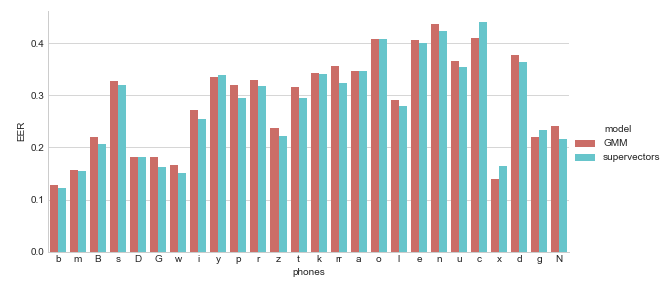
\includegraphics[width=0.8\textwidth]{files/figures/results/gmm-vs-supervectors/gmm-vs-supervectors-dev.png}
	\caption{Comparison of EER between LLR from Adapted GMMs with K-Means initialization
	and SVM trained on Supervectors for all phones in the development set, sorted
	descendently by Kappa values.}
	\label{fig:gmmSupervectorsDev}
\end{figure}

The same experiment was carried out in the heldout set leading to the results shown below.
Both systems had a very similar performance for each phoneme compared with the results obtained
in the development set, from which one can deduce that both classifiers generalize well to
unobserved data. This time, however, it was the Adapted GMM with K-Means initialization
which produced an overall weighted EER relative reduction of 0.8\% with respect to the SVMs
trained on supervectors. Even though the expected result would have been that the SVM performed
slightly better than the GMM as in \cite{main} and as it occurred in the development set,
the degradation is less than 1\% so it is still a reasonable result. In all the experiments
carried out to compare the SVMs trained on supervectors and the Adapted GMMs, both classifiers
shown a very similar performance on each phoneme.

After the successful replication of the initial experiments, a validated SVM model based on
supervectors was obtained. This classifier is used as baseline and starting point for
the next experiments,
whose objective is to analyse if an aditional gain in the performance could be achieved by
combining the supervectors features with features that carry temporal information.

\begin{figure}[H]
	\centering
	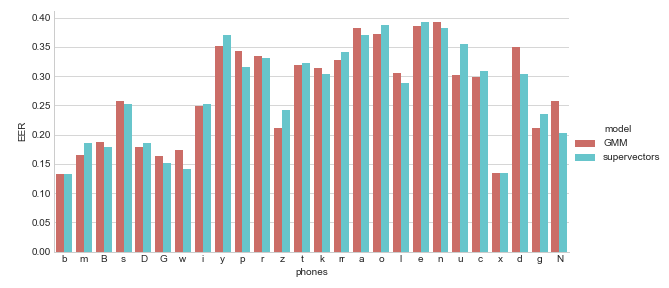
\includegraphics[width=0.8\textwidth]{files/figures/results/gmm-vs-supervectors/gmm-vs-supervectors-heldout.png}
	\caption{Comparison of EER between LLR from Adapted GMMs with K-Means initialization
	and SVM trained on Supervectors for all phones in the test set, sorted descendently
	by Kappa values.}
	\label{fig:gmmSupervectorsTest}
\end{figure}

\section{Legendre Best System}

\begin{figure}[H]
	\centering
	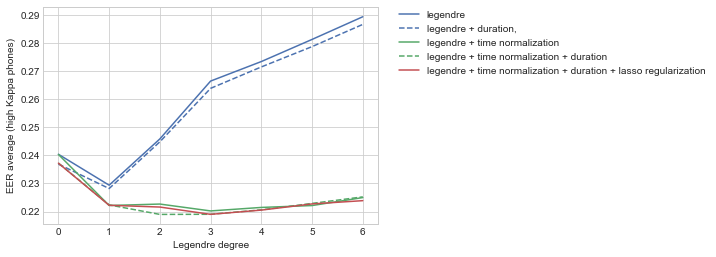
\includegraphics[width=1.0\textwidth]{files/figures/results/legendre-dct/legendre-tunning.png}
	\caption{EER average over phonemes with high Kappa for different
	degrees of Legendre Polynomials in
	the training set. Additional configurations are also studied along with the degree and
	represented by different curves: time normalization, appending the duration and applying
	Lasso Regression}
	\label{fig:legendreTunning}
\end{figure}


\section{Legendre vs DCT}

\begin{figure}[H]
	\centering
	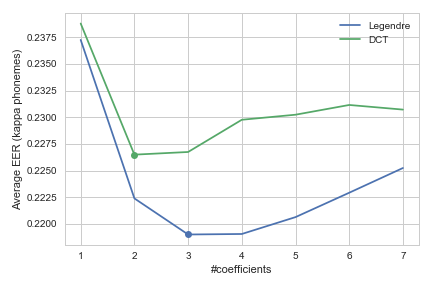
\includegraphics[width=0.5\textwidth]{files/figures/results/legendre-dct/legendre-dct-coefficients.png}
	\caption{EER average over phonemes with high Kappa as function of the number of coefficients
	for both Legendre Polynomials and DCT in the training set.}
	\label{fig:legendreVsDCT}
\end{figure}


\section{Fusion systems}

\subsection{Statistical Significant Filtering}

\subsection{Plots}

\begin{figure}[H]
	\centering
	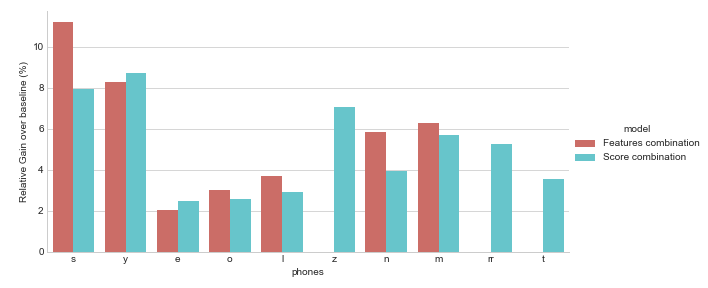
\includegraphics[width=0.8\textwidth]{files/figures/results/relatives/relatives-fusion-systems-dev-mcnemar.png}
	\caption{Comparison of performance between Features Combination system and the score combination
	of individual systems in the training set for the phones whose results were significant
	in the training set, sorted descendently by their p-value obtained in the McNemar test.
	For all the score combinations phones the results were significant in the training set,
	whereas for the features combination phones only the phones marked with (*) were significant,
	and those marked with (**) weren't significant.}
	\label{fig:fusionMcnemarDev}
\end{figure}

\begin{figure}[H]
	\centering
	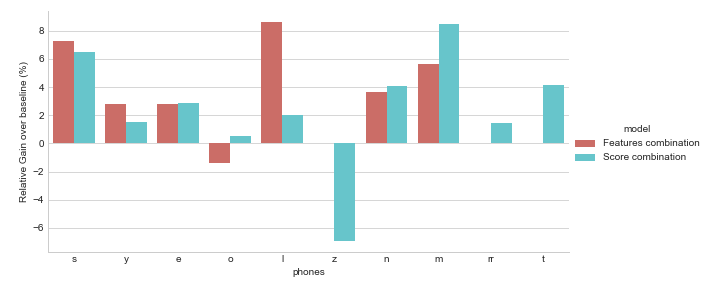
\includegraphics[width=0.8\textwidth]{files/figures/results/relatives/relative-fusion-systems-heldout-mcnemar.png}
	\caption{Comparison of performance between Features Combination system and the score combination
	of individual systems in the test set for the phones whose results were significant
	in the training set, sorted descendently by their p-value obtained in the McNemar test.
	For all the score combinations phones the results were significant in the training set,
	whereas for the features combination phones only the phones marked with (*) were significant,
	and those marked with (**) weren't significant.}
	\label{fig:fusionMcnemarTest}
\end{figure}
